\vspace{10pt}

{\centering\subsection*{何宇州:我的心爱之物}}

\addcontentsline{toc}{subsection}{何宇州:我的心爱之物}

\renewcommand{\leftmark}{何宇州:我的心爱之物}

\begin{figure}[htbp]

\centering

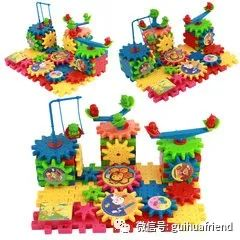
\includegraphics[width = .5\textwidth]{./ch/12.jpg}

\end{figure}



我有很多玩具,比如:遥控汽车、玩具加特林、一把木弓、一把铁做的不锐利的剑和一架遥控飞机等等。可是我最喜欢的都不是这些,我最喜欢的是乐高积木。

我的第一个乐高积木特别小,和一个修正带差不多大。它是我姑姑在武汉的一个小超市买的。它是一个小挖机的模型,是由绿色和枯黄色组成的。记得我第一次看见乐高积木时,我就深深的喜欢上了玩积木。从此我就大量的收集积木,买来之后迫不及待的先把它们拼好,然后再把它们拆了,放在一个大盒子里,自己随意拼自己想拼的模型。我拼好了自己想拼的模型,我就把它们放在柜子里展示,如果我想玩的时候再把它们拿出来,再拆再拼。

积木成了我最好的朋友!它不仅给我带来了快乐,还可以还分担我的忧愁!

如果我不高兴,积木们好像在说:“小主人不要不高兴,快来帮我们多拼一些小伙伴,到时候我们还要比赛呢!”之后我就给他们分队……

我的积木陪伴了我六年了,我是那么的喜欢他它。但是我也因为玩积木入神而被妈妈责罚。

有一次我玩积木玩的太投入,竟然忘了写作业,妈妈看见了生气的对我说:“你再这样玩,影响了学习,我要把你所有的积木都丢了。”我一听吓得目瞪口呆,赶紧求求妈妈不要丢,并答应妈妈以后要以学习为主,妈妈看我态度诚恳,就同意不丢我的积木。从那以后我再也没有因为玩积木而耽误学习。

我很喜欢我的积木朋友,它给我带来了很多快乐!





\vspace{10pt}



作者:五(3)何宇州



指导老师:刘婷



投稿:2021年6月2日



发表:2021年6月2日








                



\vspace{10pt}

\hline



